
%% bare_conf.tex
%% V1.3
%% 2007/01/11
%% by Michael Shell
%% See:
%% http://www.michaelshell.org/
%% for current contact information.
%%
%% This is a skeleton file demonstrating the use of IEEEtran.cls
%% (requires IEEEtran.cls version 1.7 or later) with an IEEE conference paper.
%%
%% Support sites:
%% http://www.michaelshell.org/tex/ieeetran/
%% http://www.ctan.org/tex-archive/macros/latex/contrib/IEEEtran/
%% and
%% http://www.ieee.org/

%%*************************************************************************
%% Legal Notice:
%% This code is offered as-is without any warranty either expressed or
%% implied; without even the implied warranty of MERCHANTABILITY or
%% FITNESS FOR A PARTICULAR PURPOSE! 
%% User assumes all risk.
%% In no event shall IEEE or any contributor to this code be liable for
%% any damages or losses, including, but not limited to, incidental,
%% consequential, or any other damages, resulting from the use or misuse
%% of any information contained here.
%%
%% All comments are the opinions of their respective authors and are not
%% necessarily endorsed by the IEEE.
%%
%% This work is distributed under the LaTeX Project Public License (LPPL)
%% ( http://www.latex-project.org/ ) version 1.3, and may be freely used,
%% distributed and modified. A copy of the LPPL, version 1.3, is included
%% in the base LaTeX documentation of all distributions of LaTeX released
%% 2003/12/01 or later.
%% Retain all contribution notices and credits.
%% ** Modified files should be clearly indicated as such, including  **
%% ** renaming them and changing author support contact information. **
%%
%% File list of work: IEEEtran.cls, IEEEtran_HOWTO.pdf, bare_adv.tex,
%%                    bare_conf.tex, bare_jrnl.tex, bare_jrnl_compsoc.tex
%%*************************************************************************

% *** Authors should verify (and, if needed, correct) their LaTeX system  ***
% *** with the testflow diagnostic prior to trusting their LaTeX platform ***
% *** with production work. IEEE's font choices can trigger bugs that do  ***
% *** not appear when using other class files.                            ***
% The testflow support page is at:
% http://www.michaelshell.org/tex/testflow/



% Note that the a4paper option is mainly intended so that authors in
% countries using A4 can easily print to A4 and see how their papers will
% look in print - the typesetting of the document will not typically be
% affected with changes in paper size (but the bottom and side margins will).
% Use the testflow package mentioned above to verify correct handling of
% both paper sizes by the user's LaTeX system.
%
% Also note that the "draftcls" or "draftclsnofoot", not "draft", option
% should be used if it is desired that the figures are to be displayed in
% draft mode.
%
\documentclass[conference]{IEEEtran}
% Add the compsoc option for Computer Society conferences.
%
% If IEEEtran.cls has not been installed into the LaTeX system files,
% manually specify the path to it like:
% \documentclass[conference]{../sty/IEEEtran}





% Some very useful LaTeX packages include:
% (uncomment the ones you want to load)


% *** MISC UTILITY PACKAGES ***
%
%\usepackage{ifpdf}
% Heiko Oberdiek's ifpdf.sty is very useful if you need conditional
% compilation based on whether the output is pdf or dvi.
% usage:
% \ifpdf
%   % pdf code
% \else
%   % dvi code
% \fi
% The latest version of ifpdf.sty can be obtained from:
% http://www.ctan.org/tex-archive/macros/latex/contrib/oberdiek/
% Also, note that IEEEtran.cls V1.7 and later provides a builtin
% \ifCLASSINFOpdf conditional that works the same way.
% When switching from latex to pdflatex and vice-versa, the compiler may
% have to be run twice to clear warning/error messages.






% *** CITATION PACKAGES ***
%
%\usepackage{cite}
% cite.sty was written by Donald Arseneau
% V1.6 and later of IEEEtran pre-defines the format of the cite.sty package
% \cite{} output to follow that of IEEE. Loading the cite package will
% result in citation numbers being automatically sorted and properly
% "compressed/ranged". e.g., [1], [9], [2], [7], [5], [6] without using
% cite.sty will become [1], [2], [5]--[7], [9] using cite.sty. cite.sty's
% \cite will automatically add leading space, if needed. Use cite.sty's
% noadjust option (cite.sty V3.8 and later) if you want to turn this off.
% cite.sty is already installed on most LaTeX systems. Be sure and use
% version 4.0 (2003-05-27) and later if using hyperref.sty. cite.sty does
% not currently provide for hyperlinked citations.
% The latest version can be obtained at:
% http://www.ctan.org/tex-archive/macros/latex/contrib/cite/
% The documentation is contained in the cite.sty file itself.






% *** GRAPHICS RELATED PACKAGES ***
%
\ifCLASSINFOpdf
  % \usepackage[pdftex]{graphicx}
  % declare the path(s) where your graphic files are
  % \graphicspath{{../pdf/}{../jpeg/}}
  % and their extensions so you won't have to specify these with
  % every instance of \includegraphics
  % \DeclareGraphicsExtensions{.pdf,.jpeg,.png}
\else
  % or other class option (dvipsone, dvipdf, if not using dvips). graphicx
  % will default to the driver specified in the system graphics.cfg if no
  % driver is specified.
  % \usepackage[dvips]{graphicx}
  % declare the path(s) where your graphic files are
  % \graphicspath{{../eps/}}
  % and their extensions so you won't have to specify these with
  % every instance of \includegraphics
  % \DeclareGraphicsExtensions{.eps}
\fi
% graphicx was written by David Carlisle and Sebastian Rahtz. It is
% required if you want graphics, photos, etc. graphicx.sty is already
% installed on most LaTeX systems. The latest version and documentation can
% be obtained at: 
% http://www.ctan.org/tex-archive/macros/latex/required/graphics/
% Another good source of documentation is "Using Imported Graphics in
% LaTeX2e" by Keith Reckdahl which can be found as epslatex.ps or
% epslatex.pdf at: http://www.ctan.org/tex-archive/info/
%
% latex, and pdflatex in dvi mode, support graphics in encapsulated
% postscript (.eps) format. pdflatex in pdf mode supports graphics
% in .pdf, .jpeg, .png and .mps (metapost) formats. Users should ensure
% that all non-photo figures use a vector format (.eps, .pdf, .mps) and
% not a bitmapped formats (.jpeg, .png). IEEE frowns on bitmapped formats
% which can result in "jaggedy"/blurry rendering of lines and letters as
% well as large increases in file sizes.
%
% You can find documentation about the pdfTeX application at:
% http://www.tug.org/applications/pdftex
\usepackage[utf8]{inputenc}
\usepackage[T1]{fontenc}
\usepackage[french, english]{babel}

\usepackage{graphicx}
\usepackage{caption}
\usepackage{amsmath,amsfonts,amssymb}
\usepackage{subcaption}


% *** MATH PACKAGES ***
%
%\usepackage[cmex10]{amsmath}
% A popular package from the American Mathematical Society that provides
% many useful and powerful commands for dealing with mathematics. If using
% it, be sure to load this package with the cmex10 option to ensure that
% only type 1 fonts will utilized at all point sizes. Without this option,
% it is possible that some math symbols, particularly those within
% footnotes, will be rendered in bitmap form which will result in a
% document that can not be IEEE Xplore compliant!
%
% Also, note that the amsmath package sets \interdisplaylinepenalty to 10000
% thus preventing page breaks from occurring within multiline equations. Use:
%\interdisplaylinepenalty=2500
% after loading amsmath to restore such page breaks as IEEEtran.cls normally
% does. amsmath.sty is already installed on most LaTeX systems. The latest
% version and documentation can be obtained at:
% http://www.ctan.org/tex-archive/macros/latex/required/amslatex/math/





% *** SPECIALIZED LIST PACKAGES ***
%
%\usepackage{algorithmic}
% algorithmic.sty was written by Peter Williams and Rogerio Brito.
% This package provides an algorithmic environment fo describing algorithms.
% You can use the algorithmic environment in-text or within a figure
% environment to provide for a floating algorithm. Do NOT use the algorithm
% floating environment provided by algorithm.sty (by the same authors) or
% algorithm2e.sty (by Christophe Fiorio) as IEEE does not use dedicated
% algorithm float types and packages that provide these will not provide
% correct IEEE style captions. The latest version and documentation of
% algorithmic.sty can be obtained at:
% http://www.ctan.org/tex-archive/macros/latex/contrib/algorithms/
% There is also a support site at:
% http://algorithms.berlios.de/index.html
% Also of interest may be the (relatively newer and more customizable)
% algorithmicx.sty package by Szasz Janos:
% http://www.ctan.org/tex-archive/macros/latex/contrib/algorithmicx/




% *** ALIGNMENT PACKAGES ***
%
%\usepackage{array}
% Frank Mittelbach's and David Carlisle's array.sty patches and improves
% the standard LaTeX2e array and tabular environments to provide better
% appearance and additional user controls. As the default LaTeX2e table
% generation code is lacking to the point of almost being broken with
% respect to the quality of the end results, all users are strongly
% advised to use an enhanced (at the very least that provided by array.sty)
% set of table tools. array.sty is already installed on most systems. The
% latest version and documentation can be obtained at:
% http://www.ctan.org/tex-archive/macros/latex/required/tools/


%\usepackage{mdwmath}
%\usepackage{mdwtab}
% Also highly recommended is Mark Wooding's extremely powerful MDW tools,
% especially mdwmath.sty and mdwtab.sty which are used to format equations
% and tables, respectively. The MDWtools set is already installed on most
% LaTeX systems. The lastest version and documentation is available at:
% http://www.ctan.org/tex-archive/macros/latex/contrib/mdwtools/


% IEEEtran contains the IEEEeqnarray family of commands that can be used to
% generate multiline equations as well as matrices, tables, etc., of high
% quality.


%\usepackage{eqparbox}
% Also of notable interest is Scott Pakin's eqparbox package for creating
% (automatically sized) equal width boxes - aka "natural width parboxes".
% Available at:
% http://www.ctan.org/tex-archive/macros/latex/contrib/eqparbox/





% *** SUBFIGURE PACKAGES ***
%\usepackage[tight,footnotesize]{subfigure}
% subfigure.sty was written by Steven Douglas Cochran. This package makes it
% easy to put subfigures in your figures. e.g., "Figure 1a and 1b". For IEEE
% work, it is a good idea to load it with the tight package option to reduce
% the amount of white space around the subfigures. subfigure.sty is already
% installed on most LaTeX systems. The latest version and documentation can
% be obtained at:
% http://www.ctan.org/tex-archive/obsolete/macros/latex/contrib/subfigure/
% subfigure.sty has been superceeded by subfig.sty.



%\usepackage[caption=false]{caption}
%\usepackage[font=footnotesize]{subfig}
% subfig.sty, also written by Steven Douglas Cochran, is the modern
% replacement for subfigure.sty. However, subfig.sty requires and
% automatically loads Axel Sommerfeldt's caption.sty which will override
% IEEEtran.cls handling of captions and this will result in nonIEEE style
% figure/table captions. To prevent this problem, be sure and preload
% caption.sty with its "caption=false" package option. This is will preserve
% IEEEtran.cls handing of captions. Version 1.3 (2005/06/28) and later 
% (recommended due to many improvements over 1.2) of subfig.sty supports
% the caption=false option directly:
%\usepackage[caption=false,font=footnotesize]{subfig}
%
% The latest version and documentation can be obtained at:
% http://www.ctan.org/tex-archive/macros/latex/contrib/subfig/
% The latest version and documentation of caption.sty can be obtained at:
% http://www.ctan.org/tex-archive/macros/latex/contrib/caption/




% *** FLOAT PACKAGES ***
%
%\usepackage{fixltx2e}
% fixltx2e, the successor to the earlier fix2col.sty, was written by
% Frank Mittelbach and David Carlisle. This package corrects a few problems
% in the LaTeX2e kernel, the most notable of which is that in current
% LaTeX2e releases, the ordering of single and double column floats is not
% guaranteed to be preserved. Thus, an unpatched LaTeX2e can allow a
% single column figure to be placed prior to an earlier double column
% figure. The latest version and documentation can be found at:
% http://www.ctan.org/tex-archive/macros/latex/base/



%\usepackage{stfloats}
% stfloats.sty was written by Sigitas Tolusis. This package gives LaTeX2e
% the ability to do double column floats at the bottom of the page as well
% as the top. (e.g., "\begin{figure*}[!b]" is not normally possible in
% LaTeX2e). It also provides a command:
%\fnbelowfloat
% to enable the placement of footnotes below bottom floats (the standard
% LaTeX2e kernel puts them above bottom floats). This is an invasive package
% which rewrites many portions of the LaTeX2e float routines. It may not work
% with other packages that modify the LaTeX2e float routines. The latest
% version and documentation can be obtained at:
% http://www.ctan.org/tex-archive/macros/latex/contrib/sttools/
% Documentation is contained in the stfloats.sty comments as well as in the
% presfull.pdf file. Do not use the stfloats baselinefloat ability as IEEE
% does not allow \baselineskip to stretch. Authors submitting work to the
% IEEE should note that IEEE rarely uses double column equations and
% that authors should try to avoid such use. Do not be tempted to use the
% cuted.sty or midfloat.sty packages (also by Sigitas Tolusis) as IEEE does
% not format its papers in such ways.





% *** PDF, URL AND HYPERLINK PACKAGES ***
%
%\usepackage{url}
% url.sty was written by Donald Arseneau. It provides better support for
% handling and breaking URLs. url.sty is already installed on most LaTeX
% systems. The latest version can be obtained at:
% http://www.ctan.org/tex-archive/macros/latex/contrib/misc/
% Read the url.sty source comments for usage information. Basically,
% \url{my_url_here}.





% *** Do not adjust lengths that control margins, column widths, etc. ***
% *** Do not use packages that alter fonts (such as pslatex).         ***
% There should be no need to do such things with IEEEtran.cls V1.6 and later.
% (Unless specifically asked to do so by the journal or conference you plan
% to submit to, of course. )


% correct bad hyphenation here
\hyphenation{op-tical net-works semi-conduc-tor}


\begin{document}
%
% paper title
% can use linebreaks \\ within to get better formatting as desired
\title{Allowing Stable Groups of Prosumers to Enter the Market through Proper Aggregation}


% author names and affiliations
% use a multiple column layout for up to three different
% affiliations
\author{\IEEEauthorblockN{Nicolas Gensollen}
\IEEEauthorblockA{CNRS SAMOVAR, \\
Institut Mines Telecom}
\and
\IEEEauthorblockN{Vincent Gauthier}
\IEEEauthorblockA{CNRS SAMOVAR, \\
Institut Mines Telecom}
\and
\IEEEauthorblockN{Michel Marot\\ and Monique Becker}
\IEEEauthorblockA{CNRS SAMOVAR, \\
Institut Mines Telecom}}

% conference papers do not typically use \thanks and this command
% is locked out in conference mode. If really needed, such as for
% the acknowledgment of grants, issue a \IEEEoverridecommandlockouts
% after \documentclass

% for over three affiliations, or if they all won't fit within the width
% of the page, use this alternative format:
% 
%\author{\IEEEauthorblockN{Michael Shell\IEEEauthorrefmark{1},
%Homer Simpson\IEEEauthorrefmark{2},
%James Kirk\IEEEauthorrefmark{3}, 
%Montgomery Scott\IEEEauthorrefmark{3} and
%Eldon Tyrell\IEEEauthorrefmark{4}}
%\IEEEauthorblockA{\IEEEauthorrefmark{1}School of Electrical and Computer Engineering\\
%Georgia Institute of Technology,
%Atlanta, Georgia 30332--0250\\ Email: see http://www.michaelshell.org/contact.html}
%\IEEEauthorblockA{\IEEEauthorrefmark{2}Twentieth Century Fox, Springfield, USA\\
%Email: homer@thesimpsons.com}
%\IEEEauthorblockA{\IEEEauthorrefmark{3}Starfleet Academy, San Francisco, California 96678-2391\\
%Telephone: (800) 555--1212, Fax: (888) 555--1212}
%\IEEEauthorblockA{\IEEEauthorrefmark{4}Tyrell Inc., 123 Replicant Street, Los Angeles, California 90210--4321}}




% use for special paper notices
%\IEEEspecialpapernotice{(Invited Paper)}




% make the title area
\maketitle


\begin{abstract}
%\boldmath

In a smart grid environment, we study coalitions formation of prosumers that aim at selling energy to the grid. It is paramount for the grid operation that the energy producers are able to sustain the grid demand in term of stability and minimum production requirement in order to enter the energy market. We design an algorithm that seeks to form coalitions that will meet both of these requirements:  a minium energy level for the coalition and a production of an uncorrelated source of energy in order to have stable production level during the course of the bidding. We proposed an algorithm that uses graph tools such as correlation graphs or clique percolation to form coalition that meet such complex constraints. We validate the algorithm against a random procedure and show that, it not only performs better in term of social welfare for the power grid, but also that it is more robust against unforeseen production variations to due to changing weather condition for instance. 


%There is a growing interest for coalitional concepts in the smart grid, spanning multiple objectives such as power losses reduction, benefits maximization or market stability... In this paper, we study coalitions of prosumers (agents that produce but also consume depending on time) which aim at selling energy to the grid. We reckon that the grid is able to specify two requirements (stability and minimum production) that enable a coalition to enter the market. Based on probability distributions of units available power, coalitions which are able to achieve low standard deviations are considered as stable coalitions. As it seems intuitively understandable that maintaining stable coalitions would be less expensive in terms of communication load than highly versatible ones, our objective consists in forming coalitions that satisfy grid requirements both in terms of stability and minimum production. Our definition of stability being implicitely linked to correlation between agents timeseries (see section \ref{sec:model}), we organize them over a correlation graph and use a variation of clique percolation to construct valid coalitions in reasonable time.
\end{abstract}
% IEEEtran.cls defaults to using nonbold math in the Abstract.
% This preserves the distinction between vectors and scalars. However,
% if the conference you are submitting to favors bold math in the abstract,
% then you can use LaTeX's standard command \boldmath at the very start
% of the abstract to achieve this. Many IEEE journals/conferences frown on
% math in the abstract anyway.

% no keywords




% For peer review papers, you can put extra information on the cover
% page as needed:
% \ifCLASSOPTIONpeerreview
% \begin{center} \bfseries EDICS Category: 3-BBND \end{center}
% \fi
% Mantegna
% For peerreview papers, this IEEEtran command inserts a page break and
% creates the second title. It will be ignored for other modes.
\IEEEpeerreviewmaketitle



\section{Introduction}
\label{sec:introduction}
% no \IEEEPARstart
One of the key ideas in the smart grid revolves around the introduction of communication means inside the power grids. This could enable complex improvements in the energy management and lead progressively to a greener energetic system \cite{Ramchurn} \cite{WuHamedHuangBook2011}. Distributed energy resources (DER) such as wind turbines or photovoltaic panels are not supposed to emerge only in remote farms, but also in residential areas. Together with electric vehicles, and demand side management tools, they will constitute the building blocks which will help to turn the today pure energy consumers into true actors of the grid operation \cite{Ramchurn}. Such agents that both consume and produce energy are ready to make concessions (appliances delays, V2G…) to ensure grid stability, and are commonly called prosumers \cite{Rathnayaka2012} \cite{Ramchurn}.

There seems to have a clear consensus on the benefit of having bidirectional communication flows between prosumers and the grid as most of the demand side management concepts have proposed such an architecture \cite{WuHamedHuangBook2011}. Nevertheless as the number of active prosumers is expected to rise, it is safe to assume there is a need for more complex communication patterns (such as coalitions) that will help to decrease the communication burden and in the mean time satisfy the multiple requirements of the power grid management. The formation of coalitions inside the smart grid environment could be applied to various types of agents such as self sufficient micro-grids \cite{Pahwa}, sizable and adjustable virtual power plants (VPP) \cite{Braun} \cite{Ramchurn}, or fleet of electric vehicles that back up the grid in some emergency situations (V2G) \cite{Ramchurn}. These are just a few use cases where the coalition of multiple agents can enhance the grid reliability and in the mean time reduce the communication burden.

In this paper, we focus on how to statistically improve the production stability by carefully forming coalitions of prosumers that have greater probability of staying in acceptable range of production. By using prediction techniques, we form coalitions that meet the contract values ranges proposed by the grid, enabling it to schedule its production accordingly. Meeting contract values for the prosumer are especially relevant in power trade conditions, where energy is traded based on day-ahead predictions. In this context, participants should try to minimize their prediction errors in order to maintain a stable state for the grid. They may even occur some penalties if the productions deviate from the initial contract values. However, it is pertinent for both side to maintain the production as stable as possible : for the prosumer, the stability (with renewable energy source) will impact its net gain, and for the power grid, it will helps to maintain its reliability.

In this paper, we seek at optimizing this tradeoff, that is forming coalitions able to announce “high contract values with high reliability”. We thus aim at:
\begin{itemize}
\item Realistic prosumers productions with renewable production sources  from real traces base from weather measure.
\item Minimizing the standard deviations of coalitions production probability distributions through the use of a proper utility function (see section \ref{sec:model})
\item Being (relatively) scalable with the number of prosumers
\end{itemize}

In more details, and as will be explained in section \ref{sec:model}, we consider agents that, depending on meteorological conditions, personal preferences, and their appliances (loads and generators), consume and produce more or less energy (using only wind turbines and PV as generators, which can be quite simply and efficiently modeled).  We used real meteorological traces (see section \ref{sec:model}) to account for seasonal and daily variations in the prosumers energetic output profiles as well as realistic geographical correlations. With these ingredients, we are able simulate the different production/consumption profiles.

In section \ref{sec:forming} As correlations play a significant role in our mechanism, we organize the prosumers in a correlation graph, a quite popular approach in market stocks clustering since \cite{Mantegna1999} (see section \ref{sec:related}). We will see that in such graphs, cliques represent structures of interest. In our settings, it means that cliques are “good” (from the utility point of view) foundations for high valued coalitions. We thereby use a modified clique percolation algorithm (see section \ref{sec:results}) that will enable us to expand the cliques as much as needed in order to form proper coalitions that fulfill grid requirements. Finally, in section \ref{sec:results} provides some results.


\section{Related Work}
\label{sec:related}

Traditionally, forming coalitions in a pool of agents can be done either in a centralized way where a single central unit is responsible for all the computations or in a distributed way where agents have only local knowledges and take actions accordingly. It is of common use to represent the situation and assess the stability of the solution by using game theoretic tools. Some papers focus on finding an optimal coalition structure giving a pool of autonomous self interested agents. In this direction, \cite{Saad2009} and \cite{Luan2014} design a distributed merge and split algorithm based on modified Pareto order with utility functions aiming at optimizing a parameter of interest such as energy losses or communication costs.

Attacking the stability issues of renewable DER, the TradeWind project \cite{Europe} simulated the impact of wind power on electricity exchange and cross-border congestions by using a flow-based market model. The idea revolves around identifying key european interconnections (already existant or not) in order "to make optimal use of the european spacial de-correlation of wind power". It was indeed shown that geographical aggregation provides smoothening effects and that the amount of prediction errors for wind power in a geographical region diminishes as the region size increases, especially for short forecast horizons.

On a narrower scale, the authors of \cite{Kota2011} study the formation of virtual power plants (VPP) composed of multiple self-interested DER. On the grid side, two requirements for the formation of virtual power plants are considered : the reliability of supply and the minimization of entities the grid has to deal with. From this, \cite{Kota2011} builds a pricing mechanism that encourages VPP to report true estimates of their aggregated production and penalizes prediction errors. A redistribution scheme of the VPP to the DER is also constructed such that the payoff allocation lies in the core of the game, meaning that no DER has an incentive to leave the coalition.

In this paper and as will be explained in section \ref{sec:model}, coalitions utilities depend on statistical properties of historical values. The goal being to form coalitions that, statistically speaking, are more likely to exhibit stable behaviors. We will see that, when it comes to the formation of the coalitions, a prosumer is completely interchangeable with the timeserie representing its available production.

The setting is thus similar with some fiancial studies on stock exchanges, where researchers tried to find relevant clusters of stocks based on their daily prices variations. The problem of clustering is usually approached by means of a similarity measure and completed by a clustering technique such as K-means or hierarchical clustering. Nevertheless, in \cite{Mantegna1999} Mantegna introduced another approach where stocks, represented by the timeseries of their daily log returns, are organized in a graph such that stocks (vertices) exhibiting similar price fluctuation patterns are close to each other. This closeness notion is formalized with a similarity measure based on Pearson correlation coefficient ($ d_{ij} = \dfrac{1}{2}\sqrt{2(1-\rho_{ij})} $ or $ d_{ij} = 1 - \rho_{ij}^{2} $ ) that enables to weight the edges of the graph. Because there is a distance between every two nodes, \cite{Mantegna1999} obtains a complete graph where precious information is flooded. In order to discard unsignificant information, \cite{Mantegna1999} used a minimum spanning tree oriented technique and achieves a hierarchical clustering of the stocks. Since then, several other filtering techniques have been proposed, such as k-nearest graphs, or $ \epsilon $-graphs, that relax the tree assumption \cite{Onnela2004}.

The idea of $\epsilon$-graphs consists in filtering edges based on their weight, only keeping edges whose weights are less than $ \epsilon $. Despite the procedure simplicity, the choice of $ \epsilon $ (or k for k-nearest graphs) is not trivial and may influence strongly the results. There is indeed to our knowledge no optimal rule for chosing $ \epsilon $. In \cite{Garas2008} and \cite{Onnela2004}, the authors studied the topological properties (average clustering, connectivity, relative number of cliques...) of the correlation graph against those of growing random graphs, depending on the threshold $ \epsilon $. One of the conclusions was that "strong links" (i.e links between strongly correlated timeseries) are responsible for clustering while "weak links" provide network connectivity.

Presented in this way, the timeseries clustering task seems very close to graph community detection. Communities in networks are indeed often seen as groups of nodes exhibiting high internal densities of links as well as a low density across communities \cite{Newmanb}. Although several techniques exists (based on different graph properties : modularity \cite{Newmanb}, edge betweeness \cite{Girvan2002}, spectrum of Laplacian \cite{Newman}...), the clique percolation algorithm \cite{Lancichinetti} uses directly this observation and the idea behind it is actually quite simple. It starts indeed by searching for cliques (a complete subgraph) in the given graph as potential community cores. Because other nodes can naturally belong to a community with a less strong connectivity requirement, the algorithm uses a fitness function that quantifies the quality (according to some criterions) of a community structure inside the graph. Expansed cliques alternatively look in their respective neighborhood, select the node that yields the best increase in fitness, and finally incorporate it. The percolation algorithm stops when seeds cease to grow or when all nodes are affected to at least one seed. At this point, some coalitions may be partially overlapping, meaning that a node can belong to multiple communities. Detection of overlapping communities is actually a very active field of research, especially in social networks where persons often belongs to several communities (family, friends, colleagues...).

The following section of this paper explains the model we built in order to obtain sufficient historical values for our prosumers, such that forming coalitions based on statistics is actually meaningfull. 

\section{Model}
\label{sec:model}

A major concern while designing our model was its ability to translate correctly realistic patterns (consumption and production) as well as realistic geographical correlations between patterns. Largely because of these reasons (but also because they are easily, and sometimes freely, available online) we chose to use meteorological traces as inputs. In this paper we used namely both french data from 2006 to 2012 sampled every 3 hours \cite{Infoclimat} (similar data for the United States covering 2010 can also be found at \cite{NCDC}). The weather stations already offer a quite good sampling of a given territory, and, with the growth of personal weather stations constantly updating data bases, the mesh becomes finer and finer. As shown in the first part of figure 1, the first step consists in discretizing the studied zone around well chosen weather stations and gathering traces for these stations. In this paper, we consider that prosumers can only produce through wind turbines and photovoltaic panels (PV). On the other hand, we built their consumption patterns according to two major cycles :
\begin{itemize}
\item \textbf{Daily cycles} : Consumption is low during night, and higher during the day with two picks in the morning and evening. Some noise is added so that prosumers have similar but not identical cycles.
\item \textbf{Seasonal cycles} : Consumption is higher in the winter because of heating and low in the summer (air conditioning is not considered). Temperature traces were the principal ingredient for modeling these cycles.
\end{itemize} 

\begin{center}
\begin{figure}
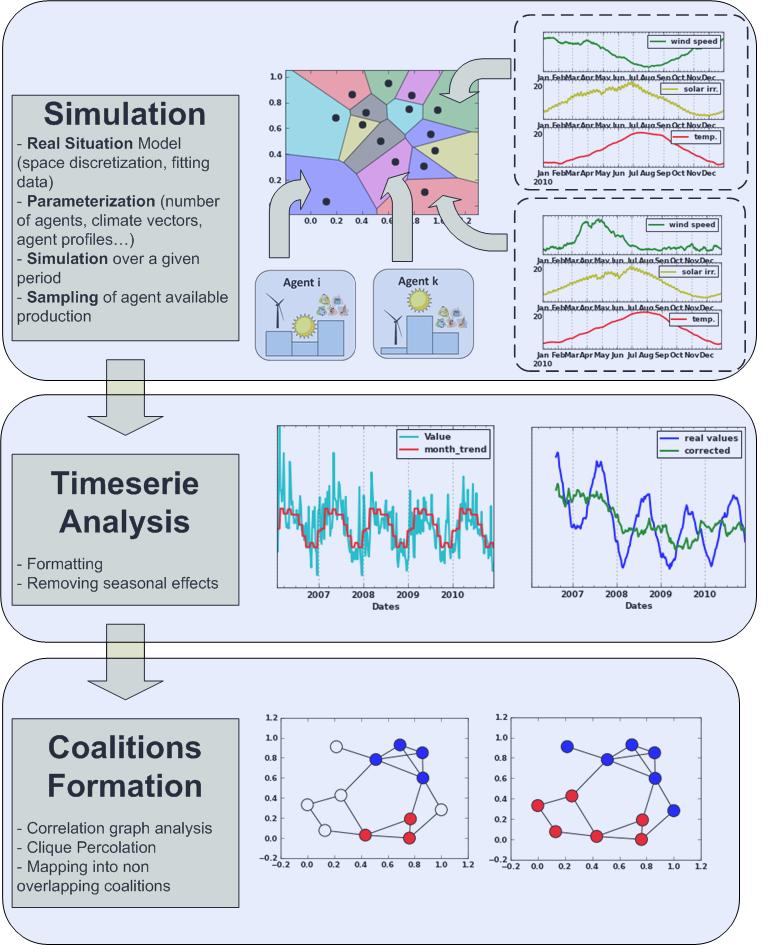
\includegraphics[scale=0.45]{figure2.jpg}
\caption{Process diagram}
\label{Fig1}
\end{figure}
\end{center}

We thus collect for all chosen weather stations three kind of traces (average wind speed, cloudiness, and average temperature), which we will call a climate vector in the following. We consider that cimate vectors are constant over their area, meaning that, if two agents are in the same area, they are exposed to the same climate vector.

At this point, modeling agents consists in fixing a few parameters (most of the time drawn from random distributions) such as the geographical position, the number of wind turbines, PV, appliances, the temperature of confort, and so on... The objective is that, depending on the weather of his zone, the DER and appliances he owns, and the way he decides to heat his home, a given prosumer is able to compute his production/consumption at any time. We thus used simple and known power curve models for linking weather variables to output power, such that a wind turbine (or a PV for instance) takes a wind speed (a solar irradiance) as input and gives an instantaneous output power \cite{Kota2011} \cite{windturbinemodel}. Any agent is thus able to compute at any time how much he produces and consumes. 


%Smart grid perspectives assume that smart meters populate the network, recording production/consumption values and reporting these to data centers. Any entities (DER, prosumers, microgrids, VPP and so on) would thereby be characterizable through timeseries expressing how much these entities produce or consume. 

%Through our model, we wish thus to be able to generate, for any prosumer, its available production over time, which depend both on its pure production and consumption. Naturally, these are far from random in the sense that there are recurring patterns (consumption or expected solar irradience for instance) or statistical properties (see wind speed studies) that shape these profiles. We thus used meteorological traces as base inputs because they naturaly provide these key ingredients (sources). On the production side, as we only consider wind turbines and photovoltaic panels as generators, we concentrate primarily on wind speed and solar irradience traces. Variables such as temperature or humidity that correlates very well with consumption were also of great use. 

%Basically, the user only has to indicate the number of prosumers and the simulation dates. Prosumers are then positioned randomly on a squared lattice. Any point of this lattice is linked to a meteorological profile derived from the input traces. A few parameters individualizing the prosumers (number and kind of DER owned, consumption habits, and so on...) are also picked randomly and account for diversity.

More formally, we denote by $ \mathcal{A} = \{ a_{1},...a_{N} \} $ the set of agents (the prosumers) and $ P_{i}(t) $ the instantaneous power value of agent i at instant t (its instantaneous production minus consumption, meaning that $ P_{i}(t) $ represents agent i available power at instant t). During the simulation (from $t_{0} $ to $ t_{K} $), all agents record their values with an hour time interval. As expected (because we introduced them), the timeseries exhibit high seasonal patterns, but completely different from agent to agent because they depend both on the energetic mix and habits of a given prosumer. Nevertheless, these macro variations can hide the interesting information in the correlation coefficients and twist the rest of our process. Thereby, we remove these seasonal effects for all agents (see second block of figure \ref{Fig1}). We denote by $ \mathcal{T}_{i} = \{ P_{i}(t_{0}),...,P_{i}(t_{K}) \} $ the resulting timeserie for  agent i. For any agent i, we note $ \mathcal{P}_{i} $ the probability distribution drawn from $ \mathcal{T}_{i} $ and by $ P_{i} $ a random variable following $ \mathcal{P}_{i} $.

We now extand these notations to any coalition $ S \subset \mathcal{A} $ : 
\begin{itemize}
\item $ P_{S}(t) = \sum_{i \in S} P_{i}(t) $
\item $ \mathcal{T}_{S} = \{ P_{S}(t_{0}),...,P_{S}(t_{K}) \} $ with $ \mathcal{P}_{S} $ its probability distribution
\item A coalition S has the possibility to announce a contract value $ P_{S}^{CRCT} $ on the market.
\end{itemize}

In this paper, we consider that coalition announcements are constrained by the grid. Namely, the grid has the possibility of fixing two parameters : 

\begin{itemize}
\item the \textbf{reliability} (denoted by $ \phi \in [0,1] $)
\item the \textbf{minimum contract value} ( $ P_{\phi}^{MIN} $). 
\end{itemize}

The reliability stipulates that for any coalition S willing to join the market, the probability of S value (at any instant t) being below its contract value should at most be $ \phi $. That is, $ \forall S,\ \forall t,\ Pr[P_{S}(t) \leq P_{S}^{CRCT} ] \leq \phi $ (for consistency we restrict $ \phi $ to small values ( $ \phi << 0.5 $)). The minimum contract value under $ \phi $ states that only coalitions with higher contract values ($ P_{S}^{CRCT} \geq P_{\phi}^{MIN} $) will be accepted.

At this point, if a coalition S whishes to join the market, it has to choose a contract value that fulfill the two conditions. For simplification, we consider that coalitions will always apply the same economically consistent strategy of announcing the highest possible contract value that obeys the reliability rule (a value we denote by $ P_{\phi}(S) $). If $ P_{\phi}(S) \geq P_{\phi}^{MIN} $, meaning that it also obeys the minimum contract value rule, then S announces this value on the market : $ P_{S}^{CRCT} = P_{\phi}(S) $. Otherwise, coalition S is not able to enter.
Basically, a coalition S is valid if and only if :
\begin{equation}
\left\{ \begin{array}{lll}
		\forall t,\ Pr[ P_{S}(t) \leq P_{\phi}(S)] \leq \phi\ \textit{{\scriptsize (reliability rule)}} \\
		and\ P_{\phi}(S) \geq P_{\phi}^{MIN}\ \textit{{\scriptsize (min value rule)}}

\end{array} \right. 
\label{rules}
\end{equation}
We now choose a very simple utility function (eq. \ref{utility}) that derives directly from the above remarks. If a coalition cannot provide a valid contract value, it receives naturally a utility of zero. Furthermore, it seems obvious that the utility should increase with the contract value. The $ 1/|S| $ term in eq. \ref{utility} indicates that we favorise small coalitions, mainly because they are easier to maintain in terms of communications.

\begin{equation}
 \mathcal{U}_{\phi,\ P_{\phi}^{MIN}}(S) = \mathbf{1}_{\textit{S\ valid}} \dfrac{P_{\phi}(S)}{|S|} 
\label{utility}
\end{equation}

Obviously, maximising this utility function amounts to maximizing the coalition contract value with the minimum possible number of agents. 

In order to illustrate what is done in the following, lets consider a very simple example with two agents, say i and j, with gaussian value probability distributions $ \mathcal{P}_{i} = \mathcal{N}(\mu_{i}, \sigma_{i}) $ and $ \mathcal{P}_{j} = \mathcal{N}(\mu_{j}, \sigma_{j}) $, such that the joint probability distribution  $ \mathcal{P}_{ij} $ of the coalition $\{ij\}$ is also a gaussian with the following parameters :

\begin{equation}
\left\{ \begin{array}{lll}
		\mu_{ij} = \mu_{i} + \mu_{j} \\
		\sigma_{ij} = \sqrt{\sigma_{i}^{2} + \sigma_{j}^{2} + \rho_{ij}\sigma_{i}\sigma_{j}}
\end{array} \right.
\label{parameters}
\end{equation}

with $ \rho_{ij} $ the Pearson correlation coefficient between $ P_{i} $ and $ P_{j} $. We can easily write the reliability condition $ Pr[P_{ij}(t) \leq P_{\phi}(ij) ] \leq \phi $ as :

\begin{equation}
\dfrac{1}{2} \left[ 1+ erf \left( \dfrac{P_{\phi}(ij) - \mu_{ij}}{\sigma_{ij}\sqrt{2}} \right) \right] \leq \phi
\label{reliability}
\end{equation}

The strategy of $ \{ij\} $ consists in maximizing its contract value as long as it respects the inequality \ref{reliability}, e.g to annonce $ P_{\phi}(ij) = \mu_{ij} - \sigma_{ij}\sqrt{2}erf^{-1}(1-2 \phi ) $. It thus appears (as it was intuitively understandable) that, for equivalent sizes, coalitions with low relative standard deviations ( $ \sigma_{ij} / \mu_{ij} $ ) are able to announce higher contract values. 

What this paper investigates in the following is the developement of an algorithm that organizes prosumers such that the synergy term of the standard deviation ( $ \rho_{ij}\sigma_{i}\sigma_{j} $ in the example above) is minimized. In such settings, and through the clique percolation procedure (section \ref{sec:forming}), we will show that coalitions with low relative standard deviation, e.g high utility coalitions, can be computed.

\section{Coalitions Formation}
\label{sec:forming}

This section explains the process with which we form the coalitions (see the third block of Figure \ref{Fig1}). First, we need to simulate the timeseries of available power (first two blocks of Figure \ref{Fig1}). We consider a pool $ \mathcal{A} $ of 200 agents, whose parameters were chosen randomly. The prosumers are positioned (also randomly) on a square lattice previously filled with climate vectors obtained from the french data sets (see section \ref{sec:model}). Simulations were run from february 2006 to december 2010 such that we are dealing with 200 hourly sampled timeseries of available power over this period. Removing season trends finally leads us to the formation of coalitions. 

The model we used in order to simulate timeseries of available production provides some diversity because of the combination between the energetic mix and the climate vectors. Nevertheless, as the number of agents grows, the timeseries tend to exhibit similar patterns. This is apparent when creating a correlation graph $ G_{1}(\mathcal{A},E_{1},\omega_{1}) $ with the same kind of metric as \cite{Garas2008} or \cite{Onnela2004} ($ d_{ij} = 1 - \rho_{ij}^{2} $), where well defined clusters appear in the $ \epsilon $-graph for any values of $ \epsilon $. 

However, these clusters of strongly correlated timeseries are the exact opposite of what we are seeking. We can indeed consider them directly as coalitions and compute their utilities, and the results show, as expected, terrible values (far worse than a random split of the agents in the same number of coalitions).

We thus opt for reversing the metric ($ d_{ij}^{'} = \rho_{ij}^{2} $) such that uncorrelated timeseries are close to each other and (anti)correlated timeseries are distant in $ G_{2}(\mathcal{A},E_{2},\omega_{2}) $. As expected \cite{Onnela2004}, independently of the $ \epsilon $ parameter, the resulting $ \epsilon $-graph exhibits henceforth much less clustering than in $ G_{1} $ and communities seem hardly visible. Therefore, using classical clustering or community detection algorithms seem to provide poor results. 

However, as seems intuitively understandable, cliques of this graph tend to exhibit very good utility values. Such  structures contain indeed a link between every two nodes, meaning that the overall correlation is quite small. Obviously, the $ \epsilon $ parameter is indirectly responsible for the sizes of the cliques, if it is too low, the $\epsilon$-graph of $ G_{2} $ will not provide enough cliques, conversely, if $\epsilon $ is too high, we loose important information as the graph becomes very dense and cliques tend to overlap strongly. For large values of $ \epsilon $ and for non trivial number of agents, finding cliques can even become computationally repulsive. Despite being direct and simple, improving the sizes of the cliques by increasing $ \epsilon $ seems too brutal. Furthermore, as the utility function is also focused on maximizing $ P_{\phi}(S) $, it might be the case that some cliques benefit from additional agents even if they don't form a clique anymore.

Cliques for small values of $ \epsilon $ appear thus as good seeds for stable coalitions, but we still have to find a way to bring them above the grid requirements as well as increasing the social welfare, both by incorporating more nodes. This is exactly where clique percolation proves useful for our concerns. The main idea of making the seeds grow as long as it increases a fitness function is exactly what we need. The only difference being that our fitness function is simply chosen as the utility function.  

As explained in section \ref{sec:related}, clique percolation leads generally to overlapping communities. For simplicity, in this paper, we wish to keep the coalitions separated and  leave the management of overlapping coalitions for future work. We thus implemented a simple heuristic that consider nodes in multiple seeds one by one and chooses its final coalition as the one that “needs it the most” in terms of utility loss. More formally, for a coalition S and a node $ i \in S $, we define :

\begin{equation}
\tau_{i}(S) = \dfrac{\mathcal{U}_{\phi,\ P_{\phi}^{MIN}}(S) - \mathcal{U}_{\phi,\ P_{\phi}^{MIN}}(S-\{i\}) }{\mathcal{U}_{\phi,\ P_{\phi}^{MIN}}(S)}
\label{tau}
\end{equation}

If node i belongs to  multiple coalitions, the only coalition retaining node i is the one that maximizes $ \tau_{i} $.

At this point, we have three degrees of freedom : the reliability ($ \phi $), the required power to enter the market ($P_{\phi}^{MIN}$), and the prunning parameter ($\epsilon$). For convenience, we introduce the number of desired coalitions ($ N_{COAL} $) and we fix $\epsilon $ as the smallest value such that the $ \epsilon $-graph contains at least $ N_{COAL} $ non overlaping cliques. The overall utility depends now on the grid requirements and on the number of desired coalitions.

The next section shows how the utility behave within the parameters space and provides the results of our 200 agents test.

\section{Results}
\label{sec:results}

\begin{center}
\begin{figure}
\setlength{\tabcolsep}{-0.7em}
\begin{tabular}{cc}
   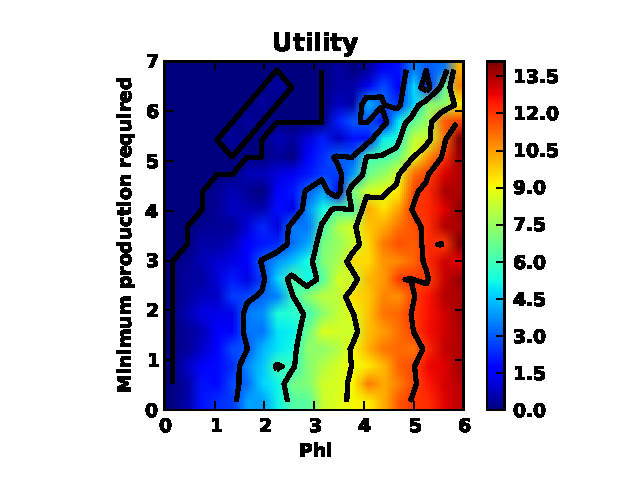
\includegraphics[scale=0.5]{./figure1/util.eps} &
   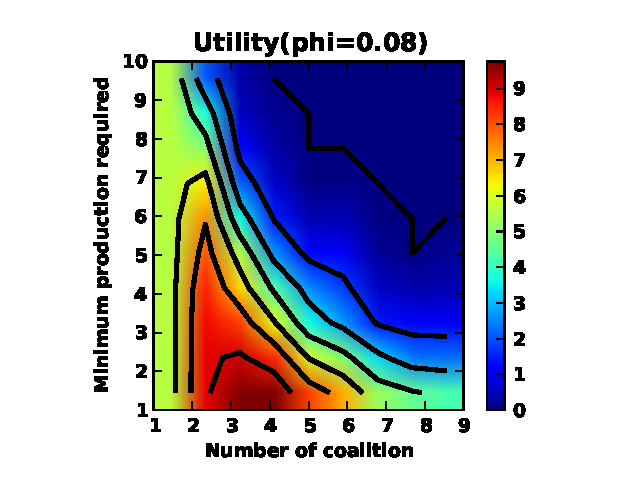
\includegraphics[scale=0.5]{./figure6/util2.eps} \\
\end{tabular}
\caption{Utility function in parameters space. Left in $ (\phi, P_{\phi}^{MIN}) $ when $ N_{COAL} $ is fixed. Right in $ (N_{COAL}, P_{\phi}^{MIN}) $ for a fixed $ \phi $}
\label{Fig2}
\end{figure}
\end{center}

As visible on the left plot of figure \ref{Fig2}, the parameters $\phi$ and $P_{\phi}^{MIN}$ shape the utility function such that, if $ \phi $ is close to zero, the reliability requirement is very high and only small values of $ P_{\phi}^{MIN}$ could potentially lead to valid coalitions (and positive utility values). Conversely, the higher $\phi$, the less constraints are imposed to the coalitions and valid ones can arise for a larger spectrum of $ P_{\phi}^{MIN}$. Obviously, the highest utility values are found for high $ \phi $, because coalitions are able then to announce higher contract values, yielding higher utilities. 

In the following, we fix the reliability to a given empirical value ($\phi = Cste $) and observe how the coalitions evolves for different values of $P_{\phi}^{MIN}$. Note that the opposite is also possible although a little less intuitive, but not shown here because of space limitations and because it leads to similar conclusions. 

On the right plot of figure \ref{Fig2}, we can see that when the grid constraints are fixed ($ \phi = 0.08 $ and $ P_{\phi}^{MIN} = 2 $ for instance) and only the number of coalitions varies, there is an increase in social welfare (sum of coalitions utilities) up to a maximum point (for $ N_{COAL} = 3 $ here) before a decrease. The reason is that increasing the number of coalitions allows more coalitions to reach stability and enter the market, but there is a point where nodes bringing stability are not sufficient inside the coalitions to make them pass the grid requirements, and some coalitions start to fail with zero utility. Moreover, reckon that increasing $ N_{COAL} $ means also increasing $ \epsilon $, leading to denser graphs where information is flooded, meaning that the algorithm performances also decrease.
Naturally, it is also visible that small values of $P_{\phi}^{MIN}$ lead to higher utilities because coalitions are able to announce higher contract values.

\begin{center}
\begin{figure}[b]
  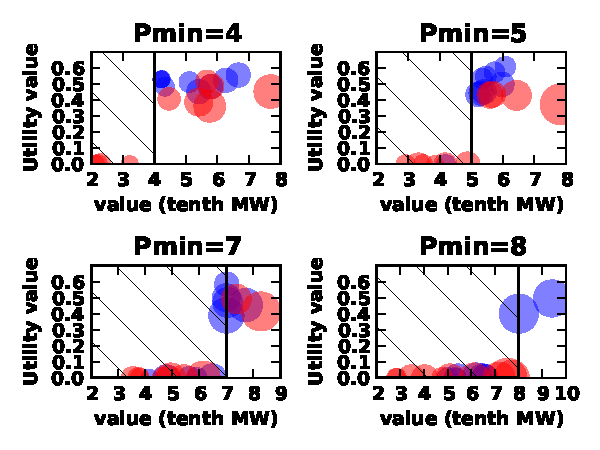
\includegraphics[scale=0.8]{./figure5/coals.pdf}
  \caption{Evolution of the coalitions for different values of $ P_{\phi}^{MIN} $ for clique percolation (blue dots) and random process (red dots).}
  \label{Fig3}
\end{figure}
\end{center}

For our 200 prosumers, we suppose that the grid fixes a reliability $ \phi = 0.1 $ (meaning that coalitions should produce more than their contract values at least $ 90 \% $ of the time). We also fix the number of coalitions to 10 and have a look at how these coalitions evolve as the grid changes the $ P_{\phi}^{MIN} $ requirement. As a comparison, we use a completely random algorithm that only asks for a number of coalitions and partitions the agents in a random fashion. Figure \ref{Fig3} shows this evolution for our algorithm (blue dots) and for the random process (red dots). The diameter of a dot is proportional to the number of agents in the coalition and the higher the dot is, the higher its utility. The $ P_{\phi}^{MIN} $ values of the x axis are expressed in tenth of MW for readability and the hatched zone corresponds to the "under-requirement space", meaning that whenever a coalition is in this zone, it has a null utility. 

Looking at figure \ref{Fig3}, we can see first that our algorithm seems to make generally a better job at finding high valued coalitions, but also that the results seem far more robust against how the grid positions its requirements. The blue dots allowed to enter the market seem indeed to outnumber the red dots, especially when the grid requirements are neither too low or too high ($ P_{\phi}^{MIN} = 5 $ in figure \ref{Fig3}).

In more details, the left plot of figure \ref{Fig4} presents the evolution of social welfare as the number of coalitions increases (all other parameters are kept constant) for both random (red curve) and clique percolation (blue curve). As for the right plot, it shows the percentage of coalitions able to enter the market for different values of $ P_{\phi}^{MIN} $. For consistency, we average the results of both plots of the random procedure over 100 realizations (5 realizations for clique percolation, but the results are relatively stable), and the errorbars in the plots stands for the standard deviations of the results.

When the grid requirements are constant (left plot), and the number of desired coalitions is low, clique percolation generally performs only a little better than random. Nevetheless, when $ N_{COAL} $ gets bigger, the performance of a random split tumble down rapidely while clique percolation social welfare decreases slowly.

When the grid requirements vary, for very low $ P_{\phi}^{MIN} $ (close to zero), all coalitions for both algorithms are able to enter the market, yielding an acceptance percentage of $ 100 \% $. But as $ P_{\phi}^{MIN} $ increases, we see the percentage of the random procedure quickly dropping while it stays constant for our algorithm. For $ P_{\phi}^{MIN} = 4 $, we see that only a little more than half of the coalitions for the random case are able to enter while all of them enters for the clique percolation algorithm. Finally, when the grid requirement becomes too high, the acceptance percentage of our algorithm tends slowly to zero (only partly shown in this plot for readability).

\begin{center}
\begin{figure}
\setlength{\tabcolsep}{0em}
\begin{tabular}{cc}
   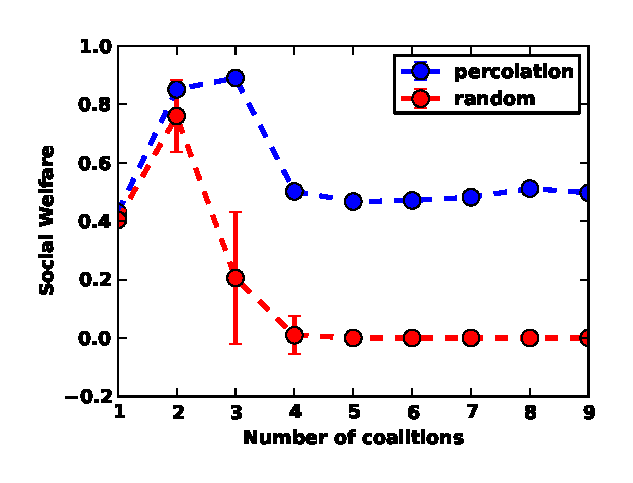
\includegraphics[scale=0.45]{./figure7/uti.eps} &
   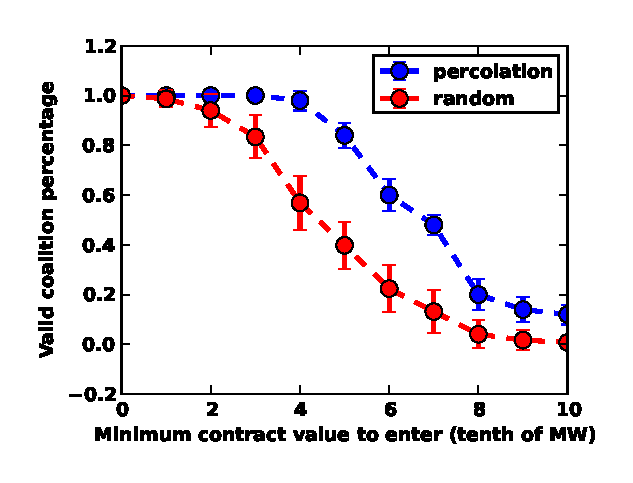
\includegraphics[scale=0.45]{./figure4/survival.eps} \\
\end{tabular}
   \caption{Percentage of coalitions able to enter the market for different values of $ P_{MIN} $ for clique percolation (blue) and random process (red).}
   \label{Fig4}
\end{figure}
\end{center}


% An example of a floating figure using the graphicx package.
% Note that \label must occur AFTER (or within) \caption.
% For figures, \caption should occur after the \includegraphics.
% Note that IEEEtran v1.7 and later has special internal code that
% is designed to preserve the operation of \label within \caption
% even when the captionsoff option is in effect. However, because
% of issues like this, it may be the safest practice to put all your
% \label just after \caption rather than within \caption{}.
%
% Reminder: the "draftcls" or "draftclsnofoot", not "draft", class
% option should be used if it is desired that the figures are to be
% displayed while in draft mode.
%
%\begin{figure}[!t]
%\centering
%\includegraphics[width=2.5in]{myfigure}
% where an .eps filename suffix will be assumed under latex, 
% and a .pdf suffix will be assumed for pdflatex; or what has been declared
% via \DeclareGraphicsExtensions.
%\caption{Simulation Results}
%\label{fig_sim}
%\end{figure}

% Note that IEEE typically puts floats only at the top, even when this
% results in a large percentage of a column being occupied by floats.


% An example of a double column floating figure using two subfigures.
% (The subfig.sty package must be loaded for this to work.)
% The subfigure \label commands are set within each subfloat command, the
% \label for the overall figure must come after \caption.
% \hfil must be used as a separator to get equal spacing.
% The subfigure.sty package works much the same way, except \subfigure is
% used instead of \subfloat.
%
%\begin{figure*}[!t]
%\centerline{\subfloat[Case I]\includegraphics[width=2.5in]{subfigcase1}%
%\label{fig_first_case}}
%\hfil
%\subfloat[Case II]{\includegraphics[width=2.5in]{subfigcase2}%
%\label{fig_second_case}}}
%\caption{Simulation results}
%\label{fig_sim}
%\end{figure*}
%
% Note that often IEEE papers with subfigures do not employ subfigure
% captions (using the optional argument to \subfloat), but instead will
% reference/describe all of them (a), (b), etc., within the main caption.


% An example of a floating table. Note that, for IEEE style tables, the 
% \caption command should come BEFORE the table. Table text will default to
% \footnotesize as IEEE normally uses this smaller font for tables.
% The \label must come after \caption as always.
%
%\begin{table}[!t]
%% increase table row spacing, adjust to taste
%\renewcommand{\arraystretch}{1.3}
% if using array.sty, it might be a good idea to tweak the value of
% \extrarowheight as needed to properly center the text within the cells
%\caption{An Example of a Table}
%\label{table_example}
%\centering
%% Some packages, such as MDW tools, offer better commands for making tables
%% than the plain LaTeX2e tabular which is used here.
%\begin{tabular}{|c||c|}
%\hline
%One & Two\\
%\hline
%Three & Four\\
%\hline
%\end{tabular}
%\end{table}


% Note that IEEE does not put floats in the very first column - or typically
% anywhere on the first page for that matter. Also, in-text middle ("here")
% positioning is not used. Most IEEE journals/conferences use top floats
% exclusively. Note that, LaTeX2e, unlike IEEE journals/conferences, places
% footnotes above bottom floats. This can be corrected via the \fnbelowfloat
% command of the stfloats package.



\section{Conclusion}
\label{sec: conclusion}

We believe that the originality of this paper lies in its willingness to exploit the de-correlation of prosumer profiles in order to build stable coalitions. In this direction, we presented a model based on meteorological traces, that captures the complex "\textit{energetic mix/climate vectors}" combination and generates realistic production and consumption patterns. We then built a framework that enables the grid to specify stability and minimum production requirements for filtering the coalitions. On this basis, we proposed a simple algorithm that seeks for uncorrelated prosumer patterns as potential seeds and expand them in coalitions able to rise above the grid requirements.

The algorithm is validated against a random process, where we show that it performs better (coalitions are more stable and the overall production is more important) and that it exhibits a higher robustness/flexibility against grid requirements changes.

%In this paper we collected meteorological traces for weather stations sampling a given territory. After discetization of the space, each zone receives the climate vector corresponding to its mother weather station. Prosumers are then distributed randomly between zones and each prosumer receives a random number of DER and loads as well as diverse consumption habits. Simulations are then runned and allow us to obtain, for each prosumer, the timeserie describing the instantaneous power that he could potentially be wanted to sell on the market. Nevertheless, as entering on the energy market is constrained by the grid operator, such that only sufficiently reliable and sufficiently productive units are allowed to enter, prosumers have usually no other choice than forming coalitions. We then introduced a framework such that the grid requirements take a precise meaning and such that coalitions announce contract values accordingly. 

%Through this paper, our interest was on how we could circumscribe groups of prosumers that can rise above the grid requirements. In this direction, we removed seasonal variations from the prosumers timeseries and proposed to organize them over a correlation graph with a reversed metric. A greedy clique percolation process on the $ \epsilon $-graph enables us to finally establish coalitions of agents. We showed in section \ref{sec:results} that our algorithm was actually finding coalitions with high utility values but also that it was far more robust than a random search over coalition structures when the grid operator increases his requirements (Figure \ref{Fig4}).

Interresting leads for future works would be the use of correlated clusters to reduce the number of entities the algorithm has to deal with, or the introduction of a payoff allocation towards the prosumers such that the stability against player defection could be analysed through game theory. Showing that maintaining the coalitions formed with our algorithm necessitates less communication and less storage capacity could also conduct to a stimulating project. Besides, we believe that not restricting the algorithm to non overlapping coalitions and studying the strategies and weights of nodes with multiple options could lead to interesting works.




% conference papers do not normally have an appendix


% trigger a \newpage just before the given reference
% number - used to balance the columns on the last page
% adjust value as needed - may need to be readjusted if
% the document is modified later
%\IEEEtriggeratref{8}
% The "triggered" command can be changed if desired:
%\IEEEtriggercmd{\enlargethispage{-5in}}

% references section

% can use a bibliography generated by BibTeX as a .bbl file
% BibTeX documentation can be easily obtained at:
% http://www.ctan.org/tex-archive/biblio/bibtex/contrib/doc/
% The IEEEtran BibTeX style support page is at:
% http://www.michaelshell.org/tex/ieeetran/bibtex/
%\bibliographystyle{IEEEtran}
% argument is your BibTeX string definitions and bibliography database(s)
%\bibliography{IEEEabrv,../bib/paper}
%
% <OR> manually copy in the resultant .bbl file
% set second argument of \begin to the number of references
% (used to reserve space for the reference number labels box)

%\begin{thebibliography}{1}

%\bibitem{IEEEhowto:kopka}
%H.~Kopka and P.~W. Daly, \emph{A Guide to \LaTeX}, 3rd~ed.\hskip 1em plus
%  0.5em minus 0.4em\relax Harlow, England: Addison-Wesley, 1999.
 
\bibliographystyle{IEEEtran}  
\bibliography{Article}

%\end{thebibliography}




% that's all folks
\end{document}


